\documentclass[12pt, a4paper]{report}

\usepackage{graphicx}
\usepackage[utf8]{inputenc}
\usepackage[russian]{babel}
\usepackage{listingsutf8}
\usepackage{textcomp}
\usepackage{float}
\usepackage{amsmath}


\lstset{inputencoding=utf8/koi8-r, breaklines=true}

% Зачем: Переопределяем стандартную нумерацию, т.к. в отчете будут только section и т.д. в терминологии TeX
\makeatletter
\renewcommand{\thesection}{\arabic{section}}
\makeatother

\begin{document}

\begin{titlepage}
	\centering{
	        \MakeUppercase{БЕЛОРУССКИЙ ГОСУДАРСТВЕННЫЙ УНИВЕРСИТЕТ} \\[0.4cm]
	
	        Факультет прикладной математики и информатики \\[0.4cm]
	        
	        \vspace{15em}
	
	        {\large\bfseries{Отчет по лабораторной работе №2\\
	        Тема: «Итерационные методы решения СЛАУ»}} \\[2cm]

	        \noindent
	        \begin{tabular}{p{0.5\textwidth}p{0.4\textwidth}}
	            & Выполнил: \\
	            & Гаргома А.\,О. \\[1cm]

	        \end{tabular}
	        \begin{tabular}{p{0.5\textwidth}p{0.4\textwidth}}
	        	& Преподаватель: \\
	        	& Горбачева Ю.\,Н. \\[1cm]
	        	
	        \end{tabular}
	
	        \vfill
	
	        {\normalsize Минск 2019}
	
	}
\end{titlepage}

\tableofcontents


\section{Постановка задачи}

Разработать программу численного решения СЛАУ $Ax = f$ методом релаксации обеспечив сходимость итерационного процесса. В качестве критерия остановки итерационного процесса использовать $\|x^{(k+1)} - x^{(k)}\|_\infty < \epsilon$, где $\epsilon = 10^{-5}$.

\section{Теория}

Метод последовательной верхней релаксации является одним из наиболее
широко используемых на практике методов для решения СЛАУ.

Рассмотрим взвешенную сумму текущего приближения и приближения,
построенного по методу Гаусса–Зейделя:

\begin{multline}
	x^{k+1}(i) = (1-\omega) x^k(i) + \frac{\omega}{a(i,i)} \left( f(i) - \sum_{j=1}^{i-1} a(i,j) x^{k+1}(j) - \sum_{j=i+1}^{n} a(i, j) x^k(j) \right), \\ i = 1, 2, \dots, n, \: k = 0, 1, 2, \dots
	\label {eq:1}
\end{multline}

При $\omega = 1$ метод релаксации (\ref{eq:1}) есть метод Гаусса–Зейделя. Иногда при
$\omega < 1$ говорят о нижней релаксации, а при $\omega > 1$ говорят о верхней релаксации.
На практике обычно $1 < \omega < 2$, так как часто именно в таких пределах
находится оптимальное значение $\omega$, обеспечивающее наиболее быструю
сходимость.



\section{Листинг программы}

\lstinputlisting[language=Python]{code/relaxation.py}

\section{Результат работы}

\begin{verbatim}
╒══════════════════╤═══════════════════════╤══════════════════╕
│                w │   Количество итераций │   Максимум-норма │
╞══════════════════╪═══════════════════════╪══════════════════╡
│ 0.20000000000000 │                  2518 │ 0.00000999310916 │
├──────────────────┼───────────────────────┼──────────────────┤
│ 0.50000000000000 │                  1079 │ 0.00000998766243 │
├──────────────────┼───────────────────────┼──────────────────┤
│ 0.80000000000000 │                   627 │ 0.00000988394922 │
├──────────────────┼───────────────────────┼──────────────────┤
│ 1.00000000000000 │                   453 │ 0.00000997930774 │
├──────────────────┼───────────────────────┼──────────────────┤
│ 1.30000000000000 │                   272 │ 0.00000996917665 │
├──────────────────┼───────────────────────┼──────────────────┤
│ 1.50000000000000 │                   178 │ 0.00000967427544 │
├──────────────────┼───────────────────────┼──────────────────┤
│ 1.80000000000000 │                    99 │ 0.00000785260049 │
╘══════════════════╧═══════════════════════╧══════════════════╛
Матрица A: 
╒═══════╤═══════╤═══════╤═══════╤═══════╤═══════╤═══════╤═══════╤═══════╤═══════╕
│ -8.92 │ -1.74 │  4.86 │  6.39 │ -3.48 │ -5.61 │ -3.03 │  1.41 │  3.44 │ -9.75 │
├───────┼───────┼───────┼───────┼───────┼───────┼───────┼───────┼───────┼───────┤
│  7.42 │ -4.82 │ -3.08 │ -4.15 │ -0.46 │ -1.17 │ -3.69 │  4.27 │  8.02 │  2.16 │
├───────┼───────┼───────┼───────┼───────┼───────┼───────┼───────┼───────┼───────┤
│  8.45 │  8.53 │ -1.48 │  9.01 │ -3.22 │ -1.35 │  0.63 │ -6.98 │  4.96 │  8.1  │
├───────┼───────┼───────┼───────┼───────┼───────┼───────┼───────┼───────┼───────┤
│ -8.99 │ -7.43 │ -1.36 │  0.83 │ -7.13 │ -9.45 │ -8.88 │ -2.99 │ -0.84 │  0.54 │
├───────┼───────┼───────┼───────┼───────┼───────┼───────┼───────┼───────┼───────┤
│  2.58 │  4.11 │  3.54 │  9.49 │ -8.27 │  5.88 │ -0.64 │  2.1  │  0.92 │ -2.2  │
├───────┼───────┼───────┼───────┼───────┼───────┼───────┼───────┼───────┼───────┤
│ -8.98 │  2.83 │ -7.89 │ -2.53 │  6.25 │  3.47 │  7.07 │ -0.12 │  4.92 │ -4.09 │
├───────┼───────┼───────┼───────┼───────┼───────┼───────┼───────┼───────┼───────┤
│ -4.69 │  0.7  │ -7.63 │  5.56 │  8.26 │  7.88 │  9.58 │  3.98 │  9.24 │ -3.08 │
├───────┼───────┼───────┼───────┼───────┼───────┼───────┼───────┼───────┼───────┤
│ -6.6  │ -2.79 │  5.31 │  8.35 │ -4.21 │  9.27 │ -5.7  │ -3.33 │ -8.3  │ -6.23 │
├───────┼───────┼───────┼───────┼───────┼───────┼───────┼───────┼───────┼───────┤
│ -9.1  │ -1.89 │ -1.43 │  7.69 │  6.8  │  8.58 │ -6.87 │ -0.98 │  2.5  │ -7.55 │
├───────┼───────┼───────┼───────┼───────┼───────┼───────┼───────┼───────┼───────┤
│ -5.98 │  2.85 │ -9.21 │ -5.96 │  8.6  │ -0.04 │ -1.88 │ -2.12 │ -1.96 │ -2.79 │
╘═══════╧═══════╧═══════╧═══════╧═══════╧═══════╧═══════╧═══════╧═══════╧═══════╛
Точность: 1e-05
\end{verbatim}
\begin{center}
\centering
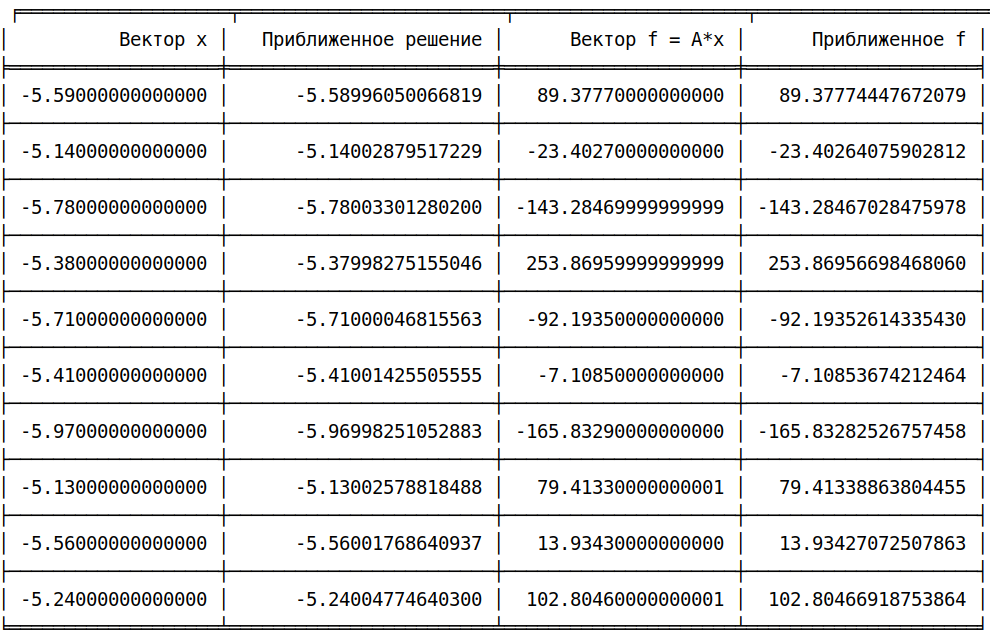
\includegraphics[scale=0.4]{images/Selection_001.png}
\end{center}
\begin{verbatim}
Максимум-норма погрешности(w = 1.8): 4.77464030019803e-05
\end{verbatim}
\section{Вывод}
Реализован алгоритм для решения СЛАУ методом релаксации.
Количество итераций уменьшается при параметре релаксации $\omega \longrightarrow 2$

\end{document}
